% This document is part of the CoordinateFree project.
% Copyright 2022 the authors.

% to-do
% -----
% - HOGG: before arXiv: switch to [preprint], add URL to colab, and uncomment the acks.
% - Soledad, BS: add grant numbers.

\documentclass{article}
% ready for submission
\usepackage{neurips_2022}

% to compile a preprint version, e.g., for submission to arXiv, add add the
% [preprint] option:
%     \usepackage[preprint]{neurips_2022}
% to compile a camera-ready version, add the [final] option, e.g.:
%     \usepackage[final]{neurips_2022}

\usepackage{wrapfig}

\usepackage[utf8]{inputenc} % allow utf-8 input
\usepackage[T1]{fontenc}    % use 8-bit T1 fonts
\usepackage{hyperref}       % hyperlinks
\usepackage{url}            % simple URL typesetting
\usepackage{booktabs}       % professional-quality tables
\usepackage{amsfonts}       % blackboard math symbols
\usepackage{nicefrac}       % compact symbols for 1/2, etc.
\usepackage{microtype}      % microtypography
\usepackage{xcolor}         % colors

\usepackage[final]{pdfpages}     % including the code at the end as supplementary

% math packages and definitions
\usepackage{amsmath}
\usepackage{amssymb}
\usepackage{tikz-cd}
\tikzcdset{every label/.append style = {font = \normalsize}}
\newcommand{\inv}{^{-1}}
\newcommand{\T}{^\top}
\newcommand{\R}{{\mathbb R}}
\newcommand{\surf}{{\mathrm{s}}}
\newcommand{\unit}[1]{\mathrm{#1}}
\newcommand{\kg}{\unit{kg}}
\newcommand{\m}{\unit{m}}
\newcommand{\s}{\unit{s}}

% text macros
\hypersetup{hidelinks}
\renewcommand{\paragraph}[1]{\par\textbf{#1}~---}
\newcommand{\bernhard}[1]{~B: \textcolor{red}{\textbf{#1}}}

\title{Representation-agnostic physics, passive symmetries,\\ and equivariant machine learning}

\author{%
  David W.~Hogg\\
 Center for Cosmology and Particle Physics, Department of Physics, New York University\\
Max Planck Institute for Astronomy, Heidelberg\\
Flatiron Institute, a Division of the Simons Foundation
  \And
George A.~Kevrekidis\\
 Department of Applied Mathematics and Statistics, Johns Hopkins University
   \And
  Bernhard Sch\"olkopf\\
  Max Planck Institute for Intelligent Systems, T\"ubingen
  \And
  Soledad Villar\\
  Department of Applied Mathematics and Statistics, Johns Hopkins University\\
  Mathematical Institute for Data Science, Johns Hopkins University
}

\frenchspacing\sloppy\sloppypar\raggedbottom
\begin{document}

\maketitle

\paragraph{Abstract} 
It has become an important goal of machine learning to develop methods that are exactly (or approximately) equivariant to group actions.
Equivariant functions obey relations like $f(g\cdot x) = g\cdot f(x)$; that is, if the inputs $x$ are transformed by group element $g$, then the outputs $f(x)$ are correspondingly transformed.
There are two different kinds of symmetries that can be encoded by these equivariances: active symmetries that are observed regularities in the laws of physics, and passive symmetries that arise from redundancies in the allowed representations of the physical objects. 
In the first category are the symmetries that lead to conservation of momentum, energy and angular momentum. In the second category are coordinate freedom, units equivariance, and gauge symmetry, among others.  
Passive symmetries always exist, even in situations in which the physical law is not actively symmetric.
For example, the physics near the surface of the Earth is very strongly oriented (free objects fall in the down direction, usually), and yet the laws can be expressed in a perfectly coordinate-free way by making use of the local gravitational acceleration vector.
The passive symmetries seem trivial, but they can lead naturally to the discovery of scalings, mechanistic structures, and missing geometric and dimensional quantities, even with limited training data.
Our conjecture is that enforcing passive symmetries in machine-learning models will improve generalization (both in and out of sample) in all areas of engineering and the natural sciences.

\section{Redundancy and passive symmetries}

In physics there are two types of symmetries. 
The first is passive symmetries, arising from the arbitrariness of the mathematical representation (including symmetries arising from coordinate freedom and equivalences of reparameterizations).
The second is active symmetries, empirically established by observations and experiments (including the symmetries that imply the fundamental conservation laws, like momentum, energy, and angular momentum). Both of these types of symmetries can be expressed in terms of group actions and equivariances, but the epistemological content and range of applicability are very different. 

The redundancies in the representations and parameterizations of the world imply a large set of symmetries.
Mathematically, this can be formulated as invariances or equivariances with respect to changes of coordinates or parameterizations (see, eg, Section 4.1 of \cite{rovelli2000loop}).
These passive symmetries include gauge freedom, units covariance, and general covariance.
These symmetries can be theoretically established with no need of observations, as they arise solely from the principle that the physical world is independent of the mathematical choices we make to describe it.
The groups involved in coordinate freedom can be large and complicated (eg, the group of reparameterizations).

In contrast to the passive symmetries, the active symmetries of the Universe are the ones that must be established experimentally.
The laws of physics do not seem (at current precision) to depend on position, orientation, or time, which in turn imply conservation of momentum, angular momentum and energy according to Noether's Theorem \cite{noether}.

Both passive and active symmetries can be illustrated by the commutative diagram \eqref{eq.diagram}. 
The space
\begin{wrapfigure}{r}{3.3cm}
\vspace{-3ex}
\begin{equation}\label{eq.diagram}
\begin{tikzcd}[]
  {\cal X}\arrow[r,"\alpha"] \arrow[d,"\Phi",swap] & {\cal X}  \arrow[d,"\Psi"]\\
{\cal H} \arrow[r,"\beta"]  & {\cal H} 
\end{tikzcd}
\end{equation}
\vspace{-3ex}
\end{wrapfigure}
$\mathcal X$ could be the space of all possible physical systems, and $\Phi$ and $\Psi$ are encodings of the systems into a space $\mathcal H$ of representations of systems (here we mean ``representation'' in the broad sense, not the group theoretic notion; see next Section).
The passive symmetries (diffeomorphisms, in the case where $\mathcal H$ is a manifold) are transformations $\{\beta:\mathcal H \to \mathcal H\}$ where $\alpha$ is taken to be the identity map.
Even in this case, there can still be different representations, because there are redundancies, or multiple elements of $\mathcal H$ that represent the same element of $\mathcal X$.\bernhard{could add: e.g., $\Phi$ and $\Psi$ might map the same physical vector to two different coordinate representations.}
The active symmetries are transformations $\{\beta:\mathcal H \to \mathcal H\}$ that preserve some important properties of the representation (element of $\mathcal H$) even when $\alpha$ is non-trivial and $\Phi\equiv \Psi$.
Because of the indifference of the physical world to mathematicians' choices, all theories are invariant with respect to passive symmetries; some (but not all) additionally have active symmetries.
%Not all contain invariances with respect to active symmetries. 

When the transformations $\alpha$ and $\beta$ are actions by a certain group, then both active and passive symmetries can be expressed in terms of group equivariances.
They are useful in machine-learning models \cite{cohen2016group, kondor2018convolution, thomas2018tensor, geiger2022e3nn, finzi2020generalizing, finzi2021practical} and have scientific applications \cite{batzner20223, musaelian2022learning, stark2022equibind, yu-physics, wang2022approximately}.
Equivariant machine-learning models can predict the properties and behaviour of physical systems (as argued in \cite{cheng2019covariance}), with the correct inductive bias, achieving smaller generalization error \cite{bietti2021sample, elesedy2021provably, elesedy2021kernel, mei2021learning} and allowing for out-of-distribution generalization \cite{villar2022dimensionless}. 
Even the non-trivial diffeomorphism symmetries of general relativity have been considered for machine learning \cite{weiler}.

The idea of homomorphic structure \eqref{eq.diagram} in the representation space $\cal H$ also applies to causal world models (eg, the brightness changes in the real world may be represented as retinal gain control mechanisms in the nervous system \cite{1911.10500}).
Other instantiations of the commutative diagram \eqref{eq.diagram} include representations that retains the dimensions of system components but drops all numbers,\bernhard{add: representations that drops the dimensions and only retains numeric values,} or the representation that converts systems into physical equations.

Most importantly, imposing a passive symmetry on the structure of a machine-learning model can permit the discovery of scalings, structures, or missing elements in the physical description of, or predictions about, the problem.
We illustrate these ideas with examples below.
The passive symmetries are seemingly trivial statements about the world, but they lead to strong constraints on the laws of physics, and deliver scaling arguments that solve real problems in physics.
They can constrain machine learning in valuable ways.
\emph{We conjecture that enforcing passive symmetries in machine learning and data-analysis tasks will lead to generalization improvements in a wide range of circumstances.}
In particular, we make this conjecture even for problems in which no (or few) active symmetries are present.
After all, most problems (like reading handwriting or predicting gravitational trajectories near the surface of the Earth) are not equivariant to rotations, reflections, and translations, but they are all, in their data-generating processes, exactly coordinate free.

Our goal is to provide definitions for these concepts and to bolster the conjecture through examples.

\section{Definitions and terminology}

\paragraph{symmetry}
Given a mathematical object $X$ of any sort, (like a manifold, metric space, equation, etc), any mapping of the object onto itself that preserves the corresponding structure is a \emph{symmetry}.

\paragraph{representation}
There are two meanings of the word \emph{representation}. One is the approximate way we describe a system (or all the objects in a system) either in a mathematical model or on a computer.
The other is the \emph{representation of a group} $G$: a homomorphism $\rho: G\to \text{GL}(V)$ where $V$ is a vector space and $\text{GL}(V)$ denotes the space of invertible linear transformations from $V$ to itself.

\paragraph{equivariance}
Let $G$ be a group that acts on vector spaces $X$ and $Y$ as $\rho_X$ and $\rho_Y$ respectively. We say that a function $f:X\to Y$ is \emph{equivariant} if for any group element $g\in G$ and any possible input $x$, the function obeys $f( \rho_X(g) x) = \rho_Y(g)\cdot f(x)$.
The actions of $G$ in $X$ and $Y$ induce an action on the space of maps from $X$ to $Y$. If $f\in \text{Maps(X,Y)}$ then $g\cdot f = \rho_Y(g)\circ f \circ \rho_X(g)^{-1}$.
The equivariant maps are the fixed points of this action.
Equivariances define symmetries in the space of maps. 

\paragraph{invariance}
\emph{Invariance} is an equivariance in which the action in the output space is trivial.

\paragraph{coordinate freedom}
When physical quantities are measured, or represented in a computer, they must be expressed in some coordinate system.
The redundancy of this representation---the fact that the investigator had many choices for the coordinate system---leads to a symmetry, which is known as \emph{coordinate freedom}:
If the inputs to a physics problem are moved to a different coordinate system (because of a change in the origin or orientation), the outputs of the problem must be correspondingly moved.

\paragraph{geometric principle}
A consequence of coordinate freedom is that the laws of physics obey a \emph{geometric principle} \cite{mcp}, according to which the laws of physics must be described in terms of scalars, vectors, and tensors.
These scalar, vector, and tensor quantities may only be combined in certain ways, encoded in detail by the Ricci--Levi-Civita (or Einstein) summation rules \cite{ricci, einstein}; see also \cite{villar2021scalars}.

\paragraph{covariance}
When a physical law is written in a way that is consistent with the geometric principle, then the law is sometimes said to be \emph{covariant}.

\paragraph{general covariance}
The covariance of relevance in general relativity \cite{einstein} is known as \emph{general covariance}.
Because general relativity is a metric theory in $3+1$ spacetime dimensions with invariance with respect to arbitrary diffeomorphisms, this is a very strong symmetry.
General covariance is sometimes called ``coordinate freedom'', but it is a special case thereof.

\paragraph{conservation law}
We say that a quantity obeys a \emph{conservation law} if changes in that quantity (with time) inside some closed volume can are quantitatively explained by fluxes of that quantity through the surface of that volume.
\emph{Active} (not passive) symmetries lead to conservation laws in dynamical systems \cite{noether}.

\paragraph{units}
All physical quantities are measured with a system of what we call \emph{units}.
A quantity can be transformed from one unit system to another by multiplication with a dimensionless number.
Almost all quantities---including almost all scalars, vectors, and tensors---have units.

\paragraph{dimensions}
The equivalence classes of quantities with units are called \emph{dimensions}.
For example, all quantities that have units that can be converted (by multiplication by a dimensionless number) to units of $\kg$ have dimensions of mass.

\paragraph{units covariance}
The left-hand side and the right-hand side of any equation must have the same units.
This symmetry is called (by us) \emph{units covariance} (contra \cite{villar2022dimensionless}).

\paragraph{gauge freedom}
Some physical quantities in field theories (for example the vector potential in electromagnetism) have additional degrees of freedom that go beyond the choice of coordinate system and units.
These freedoms lead to additional symmetries which are known as \emph{gauge freedom}.

\section{Examples}

\paragraph{Free body in gravity}
Consider a mass $m$ near the surface of the Earth, in a location where the surface of the Earth can be considered as a horizontal plane, and close enough to the surface such that the gravitational field can be considered to be determined by a constant (not spatially varying) vector with magnitude $g$ and direction downwards.
\textsl{Question~1:}~If this mass $m$ is dropped (released at rest) from a small height $h$ from above the ground, how much time $T$ does it take to fall to the ground?
\textsl{Question~2:}~If this mass $m$ is launched from the surface at a low velocity of magnitude $v$ at an angle $\theta$ to the horizontal, how much horizontal distance $L$ will it fly before it hits the surface again?
Assume that only $m, g, h$ come in to the solution; assume that the height $h$ and the velocity $v$ are both small enough that air resistance, say, can be ignored. We shall return to this seemingly innocuous point below.

The answers to these questions, it turns out, are almost completely determined by dimensional (or units-covariance) arguments.
The mass $m$ has units of $\kg$, the gravitational acceleration magnitude $g$ has units of $\m\,\s^{-2}$, the velocity magnitude $v$ has units of $\m\,\s^{-1}$, the time $T$ has units of $\s$, and the lengths $h$ and $L$ have units of $\m$.
The angle $\theta$ is dimensionless (it can be measured in radians or degrees, say, which can be converted to radians by a dimensionless constant).
The only possible combination of $m, g, h$ that has units of time is $\alpha\,\sqrt{h/g}$, where $\alpha$ is a dimensionless constant, which doesn't depend on any of the inputs.
The only possible combination of $m, g, v, \theta$ that has units of length is $\beta(\theta)\,v^2/g$, where $\beta(\theta)$ is a dimensionless function of only one dimensionless input.
That is, both Questions~1 and 2 can be answered up to a dimensionless constant (or function) without any considerations beyond those of the units of the inputs and outputs, and absolutely no training data.
And both of those answers don't depend in any way on the input mass $m$, which is the symmetry or invariance that led to the discovery of general relativity \cite{gr}.

This shows that the fundamental structure of physical law can sometimes be inferred from units covariance only, which is a passive symmetry.  Related ideas are explored in \cite{villar2022dimensionless}.

We note also that these arguments may contain information pertaining to the (hard problem of) inference of causal structure:
treating $g$ as a constant, we can construct a structural causal model with the following vertices: (a)~an initial value of $v$, (b)~a value of $m$, chosen independently, and (c)~a final value of $L$, affected by a noise term $\theta$.
Time ordering implies that possible causal arrows are from $v, m, \theta$ to $L$.
As argued above, dimensional analysis rules out the arrow $m\to l$, leaving us with the non-trivial result that in the causal graph, only $v,\theta$ cause $L$.
Again, this conclusion can be reached without training data.

\bernhard{New: There is another intriguing connection to causality that we have glossed over above.
We made the assumption that only quantities come into the solution (in our case, $m, g, h$). How would we ascertain such an assumption in practice? In essence, this is not a probabilistic statement, but one about the behavior of a system under experimentation, i.e., intervention. A set of experiments can indicate that a certain outcome (or effect variable) depends on a certain set of input (cause) variables but is independent of certain other potential cause variables. The physical law is thus not inferred from dimensional arguments alone, but from a combination of dimensional and causal arguments.}

\paragraph{Black-body radiation}
An important moment in the history of physics was the discovery by Planck that the electromagnetic radiation intensity $B_\lambda$ (energy per time per area per solid angle per wavelength) of thermal black-body radiation can be described with a simple equation \cite{planck}
\begin{equation}
    B_\lambda(\lambda) = \frac{2\,h\,c^2}{\lambda^5}\,\frac{1}{\exp\frac{h\,c}{\lambda\,k\,T} - 1}~,
\end{equation}
where $h$ is Planck's constant,
$c$ is the speed of light,
$\lambda$ is the wavelength of the electromagnetic radiation,
$k$ is Boltzmann's constant,
and $T$ is the temperature.
In finding this formula, Planck had to posit the existence (and units) of the constant $h=6.6\times 10^{-34}\,\kg\,\m^2\,\s^{-1}$ (his original value was presented with different units, but the same dimensions).
Prior to Planck's introduction of $h$, the only dimensionally acceptable expression for the black-body intensity was $B_\lambda(\lambda)=2\,c\,k\,T/\lambda^4$, which is the long-wavelength (infrared) or high-temperature limit.
Planck's discovery was important because it solved the ``ultraviolet catastrophe'' of classical physics and seeded the theory of quantum mechanics.

This problem can be solved almost directly with the passive symmetry of units covariance.
That is, the exponential cut-off of the intensity appears at a wavelength set by the temperature and a new constant, that must have units of action (or action times $c$, or action divided by $k$, or one of a restricted set of other options).
We have shown (see notebook in supplementary material), with a simple toy training set, that no units-covariant regression for the intensity as a function of $\lambda, T, c, k$ can reproduce accurately the intensity $B_\lambda$, but that when the regression is permitted to introduce a new dimensional constant (but remain units covariant given the new constant), it finds a constant with units (and, less precisely, magnitude) that is consistent with $h$ (or $h$ times a combination of $c$ and $k$).
Again, this shows that the passive symmetry leads to powerful capability.

\paragraph{Springy double pendulum}
The double pendulum connected by springs is a toy example often used in equivariant machine-learning demonstrations \cite{finzi2021practical,yao2021simple}. 
The final conditions (position and velocities of both masses after elapsed time $T$) are related to the initial conditions (position and velocities of the masses at the initial time), and the dynamics is classically chaotic.
The vectors are 3-dimensional, subject to a passive $O(3)$ equivariance, but the problem contains an \emph{active} $O(2)$ equivariance (the dynamics is equivariant with respect to rotations and reflections in the 2-d plane normal to gravity).
It was shown in \cite{yao2021simple} that when the problem is treated with a machine-learning method that is restricted to be coordinate free for the full passive $O(3)$ symmetry, training and generalization are improved over the case in which the method is restricted only to be equivariant for the smaller active $O(2)$ symmetry.
That is, even though the dynamics of the double pendulum contains an explicit spatial anisotropy, the existence of the passive $O(3)$ symmetry is powerful for model structure and generalization.
Indeed, the passive symmetry is more powerful than the active symmetry.

In that problem, $O(3)$ symmetry was implemented by converting the network inputs (which are scalars and components of vectors) into invariant scalar quantities according to the Einstein summation rules (which explicitly encode $O(3)$ symmetry), building the nonlinear machine-learning model in the space of the invariant scalars, and multiplying back to input vectors to make the output predictions (as per \cite{villar2021scalars}).
That is, the machine-learning model was restricted to use structures that are invariant to the $O(3)$ group action.
This restriction on model capacity is significant, even though the problem does not have $O(3)$ symmetry in the active sense.
Later, the passive symmetry of units covariance was also applied to this problem, and generalization improved even further \cite{villar2022dimensionless}.

\section{Implications and broader impacts}

The passive symmetries we discuss in this Note---and the consequences they generate for machine learning---apply to essentially all problems in the natural sciences, and many apply also in the social sciences (think, eg, of units covariance).
This means that symmetry-respecting model structures for machine learning will have impacts across the sciences, reducing model capacity at fixed complexity, reducing training burdens, and improving generalization.
We also conjecture that they will limit the susceptibility of these models to many kinds of adversarial attacks, because they reduce model capacity in bad parts of model space.

The practical implementations of these ideas often involve only restructuring the inputs to be invariants of the relevant group actions.
That is, these passive symmetries are not only powerful for machine learning but they are also straightforward to implement across many settings.
For these reasons the cost of implementation is low, while the benefit is high.

% \paragraph{Acknowledgments}
% It is a pleasure to thank Roger Blandford (Stanford), Jorge S.~Diaz (BASF), and Kate Storey-Fisher (NYU) for valuable comments.
% Some of this work was performed at Schloss Dagstuhl seminar 22382 on Machine Learning in the Sciences in 2022 September.

\bibliographystyle{plain}
\raggedright
\bibliography{coordinatefree}

\end{document}

\newpage
\section*{Checklist}


%%% BEGIN INSTRUCTIONS %%%
% The checklist follows the references.  Please
% read the checklist guidelines carefully for information on how to answer these
% questions.  For each question, change the default \answerTODO{} to \answerYes{},
% \answerNo{}, or \answerNA{}.  You are strongly encouraged to include a {\bf
% justification to your answer}, either by referencing the appropriate section of
% your paper or providing a brief inline description.  For example:
% \begin{itemize}
%   \item Did you include the license to the code and datasets? \answerYes{See Section~\ref{gen_inst}.}
%   \item Did you include the license to the code and datasets? \answerNo{The code and the data are proprietary.}
%   \item Did you include the license to the code and datasets? \answerNA{}
% \end{itemize}
% Please do not modify the questions and only use the provided macros for your
% answers.  Note that the Checklist section does not count towards the page
% limit.  In your paper, please delete this instructions block and only keep the
% Checklist section heading above along with the questions/answers below.
%%% END INSTRUCTIONS %%%


\begin{enumerate}


\item For all authors...
\begin{enumerate}
  \item Do the main claims made in the abstract and introduction accurately reflect the paper's contributions and scope?
    % \answerTODO{}
    \answerYes{}
  \item Did you describe the limitations of your work?
    % \answerTODO{}
    \answerYes{}
  \item Did you discuss any potential negative societal impacts of your work?
    % \answerTODO{}
    \answerNA{}
  \item Have you read the ethics review guidelines and ensured that your paper conforms to them?
    % \answerTODO{}
    \answerYes{}
\end{enumerate}


\item If you are including theoretical results...
\begin{enumerate}
  \item Did you state the full set of assumptions of all theoretical results?
    % \answerTODO{}
    \answerYes{}
        \item Did you include complete proofs of all theoretical results?
    % \answerTODO{}
    \answerNA{}
\end{enumerate}


\item If you ran experiments...
\begin{enumerate}
  \item Did you include the code, data, and instructions needed to reproduce the main experimental results (either in the supplemental material or as a URL)?
    % \answerTODO{}
    \answerYes{}
  \item Did you specify all the training details (e.g., data splits, hyperparameters, how they were chosen)?
    % \answerTODO{}
    \answerYes{}
        \item Did you report error bars (e.g., with respect to the random seed after running experiments multiple times)?
    % \answerTODO{}
    \answerNA{}
        \item Did you include the total amount of compute and the type of resources used (e.g., type of GPUs, internal cluster, or cloud provider)?
    % \answerTODO{}
    \answerYes{}
\end{enumerate}


\item If you are using existing assets (e.g., code, data, models) or curating/releasing new assets...
\begin{enumerate}
  \item If your work uses existing assets, did you cite the creators?
    % \answerTODO{}
    \answerNA{}
  \item Did you mention the license of the assets?
    % \answerTODO{}
    \answerNA{}
  \item Did you include any new assets either in the supplemental material or as a URL?
    % \answerTODO{}
    \answerYes{}
  \item Did you discuss whether and how consent was obtained from people whose data you're using/curating?
    % \answerTODO{}
    \answerNA{}
  \item Did you discuss whether the data you are using/curating contains personally identifiable information or offensive content?
    % \answerTODO{}
    \answerNA{}
\end{enumerate}


\item If you used crowdsourcing or conducted research with human subjects...
\begin{enumerate}
  \item Did you include the full text of instructions given to participants and screenshots, if applicable?
    % \answerTODO{}
    \answerNA{}
  \item Did you describe any potential participant risks, with links to Institutional Review Board (IRB) approvals, if applicable?
    % \answerTODO{}
    \answerNA{}
  \item Did you include the estimated hourly wage paid to participants and the total amount spent on participant compensation?
    % \answerTODO{}
    \answerNA{}
\end{enumerate}


\end{enumerate}

% \clearpage
% \pagebreak
% \hspace{0pt}
% \vfill
% \begin{center}
%     \textsc{Supplemental Material}: \texttt{Python} Notebooks
% \end{center}
% \vfill
% \hspace{0pt}
% \pagebreak

% 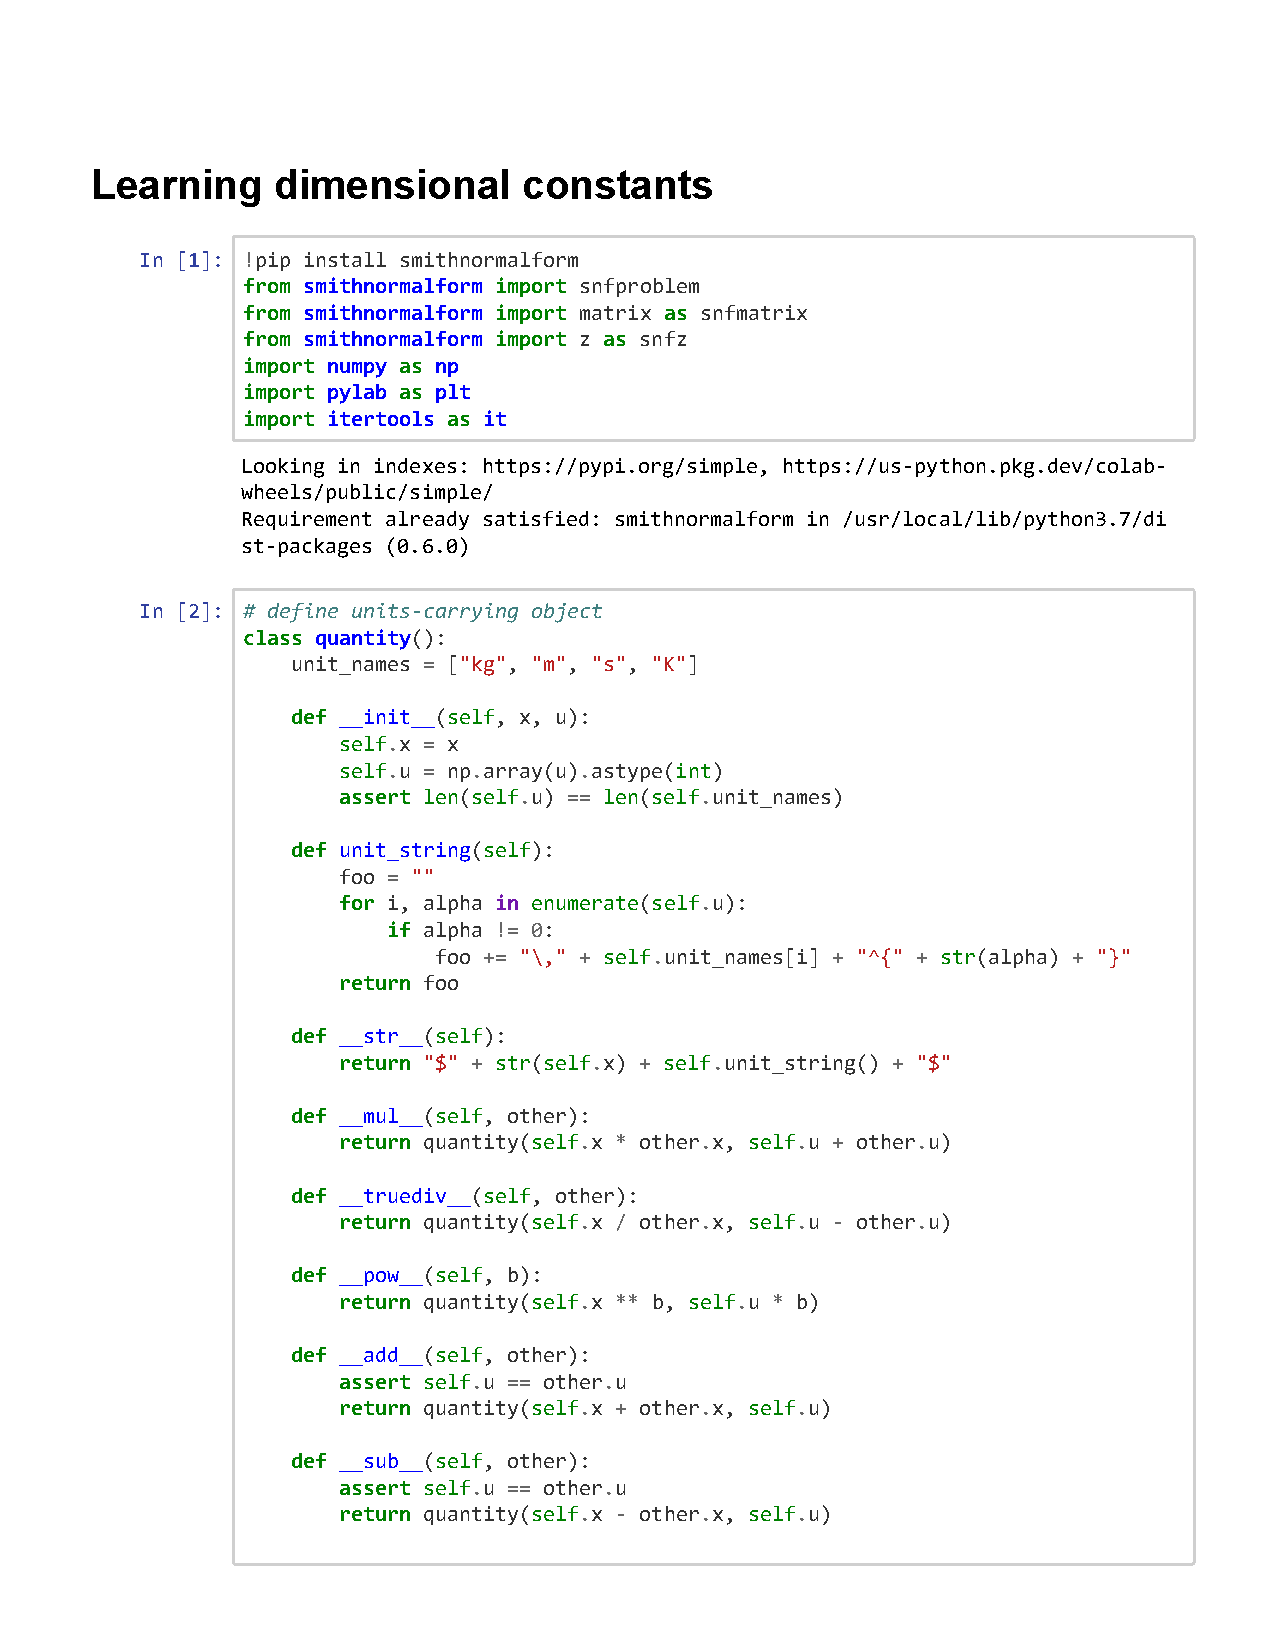
\includepdf[pages=1-12]{Learn dimensional constants.ipynb - Colaboratory.pdf}


\end{document}

% IT'S OVER
% ------------------------------------
% \section{DELETE THIS SECTION: Discussion and other random notes}

% Four special cases:
% \begin{enumerate}
%     \item the representation that retains dimensions but drops all numbers --- here the structure $\rho(g)$ is the graded algebra of dimensions...
%     \item the representation that discards all dimensions and just describes transformations of numerical quantities
%     \item a statistical representation --- here, $g$ could be 'prediction', and we may for instance want a $\Phi$ which makes prediction statistically or computationally easier
%     \item a causal representation --- here, $g$ could be a class of interventions, possibly described by a group (e.g., translations of objects)
% \end{enumerate}

% xxx could also talk about equivariance with respect to sample size. Statistical inference procedures should be expressed s.t.\ they work independent of sample size

% Approximate symmetries and representations that are approximate.

% Any connection between this stuff and causality?
% Example of cannon ball where influence of $m$ can be ruled out based on dimensional analysis --- write an SCM: (1) two variables are the initial values of $v$, $m$, chosen independently, and the final value of $l$ (2) $g$ is considered constant, (3) $\theta$ is the noise affecting $l$. From time constraints we know that the only possible causal arrows are from $v, m$ to $l$. From dimensional analysis, the arrow $m\to l$ is excluded, so we have identified the causal graph $v\to l$.


